\documentclass{article}
\usepackage[utf8]{inputenc}
\usepackage{lmodern}
\usepackage{titlesec}
\usepackage{listings}
\usepackage{xcolor}
\usepackage{minted}
\usepackage{graphicx}

\graphicspath{{img/}}

\titlespacing*{\section}      {0em}{1.25em}{.75em}
\titlespacing*{\subsection}   {0em}{1em}{.5em}
\titlespacing*{\subsubsection}{0em}{.75em}{.5em}
\titlespacing*{\paragraph}    {0em}{.50em}{.5em}
\setlength\parindent{0pt}
\setlength{\parskip}{1mm}

\newcommand{\newlineparagraph}[1]{\paragraph{#1}\mbox{}\\}
\newcommand{\twodashes}{\texttt{-{}-}}

\colorlet{punct}{red!60!black}
\definecolor{delim}{RGB}{20,105,176}
\colorlet{numb}{magenta!60!black}

\lstset{
    basicstyle=\normalfont\ttfamily,
    showstringspaces=false
}

\lstdefinelanguage{json}{
    basicstyle=\normalfont\ttfamily,
    showstringspaces=false,
    breaklines=true,
    frame=single,
    literate=
     *{0}{{{\color{numb}0}}}{1}
      {1}{{{\color{numb}1}}}{1}
      {2}{{{\color{numb}2}}}{1}
      {3}{{{\color{numb}3}}}{1}
      {4}{{{\color{numb}4}}}{1}
      {5}{{{\color{numb}5}}}{1}
      {6}{{{\color{numb}6}}}{1}
      {7}{{{\color{numb}7}}}{1}
      {8}{{{\color{numb}8}}}{1}
      {9}{{{\color{numb}9}}}{1}
      {:}{{{\color{punct}{:}}}}{1}
      {,}{{{\color{punct}{,}}}}{1}
      {\{}{{{\color{delim}{\{}}}}{1}
      {\}}{{{\color{delim}{\}}}}}{1}
      {[}{{{\color{delim}{[}}}}{1}
      {]}{{{\color{delim}{]}}}}{1},
}

\title{Simulation einer Datenübertragung mit LEB128}
\author{Michael Domanek}
\date{Jänner 2021}

\begin{document}

\maketitle

\newpage

\tableofcontents

\newpage

\section{Aufgabenstellung}
Simulation einer Datenübertragung von ganzen Zahlen basierend auf der Kodierung Signed LEB128 wobei Zahlen (zufällig zwischen ‐100000 und 100000; über die Kommandozeile konfigurierbar) zwischen zwei Threads übertragen werden sollen. Es sollen permanent Zahlen im Sekundentakt übertragen werden, wobei die Übertragung als String stattfinden soll. Es sind promise und future Paare zur Kommunikation zu verwenden.

\section{Einleitung}
In meinem Projekt geht es darum Dezimalzahlen zwischen 2 Threads zu übertragen.
Dafür wird die Dezimalzahl in unsigned/signed LEB128 kodiert dann übertragen und dann wieder zurück konvertiert.

Um die Zahlen zu unsigned LEB128 zu kodieren wurde folgendes Schema\footnote{Schema aus ihrer pdf 21\_encoding S. 6 verwendet} verwendet: 
\begin{enumerate}
\item Zahl binär darstellen
\item 0en bis auf Vielfaches von 7 links auffüllen
\item in 7er Gruppen teilen
\item auf 8 Bits bringen: MSB setzen in jeder Gruppe außer der höchstwertigsten
\item Daten beginnend mit dem niederwertigsten Byte übertragen
\end{enumerate}

Um die Zahlen zu signed LEB128 zu kodieren wurde folgendes Schema\footnote{Schema aus ihrer pdf 21\_encoding S. 8 verwendet} verwendet: 
\begin{enumerate}
\item Zahl binär darstellen (negativ → positiv, 0 Bit hinzu, 2er-Komplement)
\item VZ bis auf Vielfaches von 7 links auffüllen
\item in 7er Gruppen teilen
\item auf 8 Bits bringen: MSB setzen in jeder Gruppe außer der höchstwertigsten
\item Daten beginnend mit dem niederwertigsten Byte übertragen
\end{enumerate}

Für die Übertragung zwischen den Threads wurden promise und future Paare verwendet.
Die LEB128 kodierten zahlen werden als Strings übertragen.
\pagebreak

Im folgenden Code sieht man verkürzt wie das Programm und die Übertragung funktioniert:

\begin{minted}{c++}
LEB128 leb128{logger};

while (true) {
    promise<string> promise;
    future<string> future{promise.get_future()};
    
    thread t1{[&]{
        value = gen(rd);
        binary = leb128.toSignedLeb128(value);
        promise.set_value(binary);
        this_thread::sleep_for(chrono::milliseconds(delay));
    }};
    
    thread t2{[&]{
        string binary = future.get();
        value = leb128.signedLeb128toDecimal(binary);
        cout << value << endl;
    }};
}

t1.join();
t2.join();
\end{minted}

\section{Parameter des Komandozeileinterface}

\begin{figure}[h]
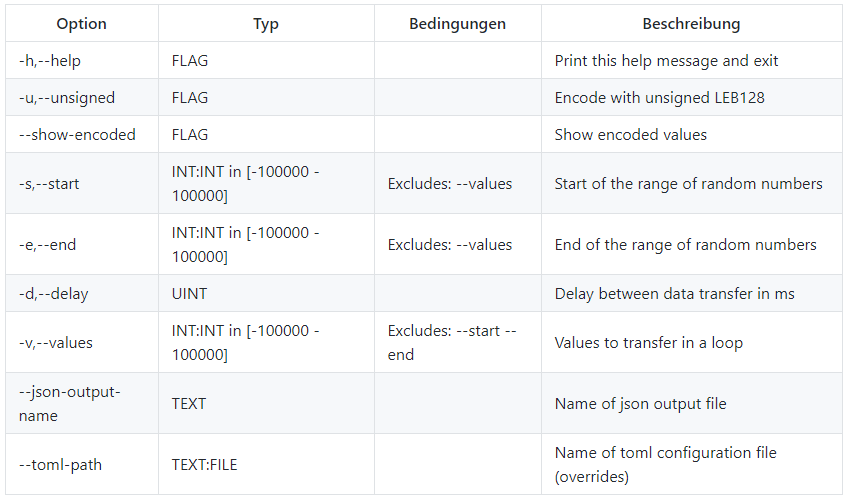
\includegraphics[width=\linewidth]{clioptions}
\caption{Eine Übersicht der Optionen der CLI}
\label{fig:clioptions}
\end{figure}

In diesem Kapitel geht es darum welche Option das Komandozeileinterface hat. 
Im Bild \ref{fig:clioptions} sieht man eine Übersicht der Optionen.

Standartmäßig werden zufällige Zahlen alle 1000ms zwischen -100000 und 100000 übertragen und die signed LEB128 Kodierung verwendet.

\newlineparagraph{\twodashes help}
Eine Ausgabe alle Komandozeilenoptionen wie in der Übersicht.
\newlineparagraph{\twodashes unsigned}
Es wird die unsigned LEB128 Kodierung verwendet.
\newlineparagraph{\twodashes show-encoded}
Es werden die Kodierten Zahlen in die Kommandozeile ausgegeben.
\newlineparagraph{\twodashes start \& \twodashes end}
Mit diesen Optionen wird der Bereich der Zufallszahlen festgelegt. Dieser muss zwischen -100000 und 100000 liegen. Beides müssen ganzahlige Werte sein und die Option \textbf{\twodashes values} darf nicht verwendet werden.
\newlineparagraph{\twodashes values}
Damit können Werte eingeben werden, die dann wiederholt übertragen werden. Für diese Werte gelten die selben Bedingungen wir für start und end. 
\newlineparagraph{\twodashes delay}
Damit wird der Dauer zwischen den Übertragungen in Millisekuden angegeben.
\newlineparagraph{\twodashes json-output-name}
Mit dieser Option legt man fest das ein JSON Datei erstellt wird mit dem angegeben Namen.
In diesem JSON stehen die Konigurationsparameter und die übergeben Werte von thread 1 und die erhaltenen Werte von thread 2.
\newlineparagraph{\twodashes toml-path}
Damit wird ein Pfad des Konfigurationsfiles festgelegt, das in TOML Syntax muss sein. Mit dieser Datei kann man alle oberhalb genannten Option festlegen bzw. man überschreibt sie wenn sie per Kommandozeile eingestellt wurden.

\section{Implementierung}
Die Implementierung des Hauptprogramms wurde großteils schon beschrieben. Zuerst werden die Kommandozeilenoptionen eingelesen und verarbeitet. Wenn irgendeine Bedingung nicht erfüllt wird, wird ein ValidationError geworfen und geloggt. In dem Programm werden entweder Zufallszahlen oder die Werte von \textbf{\twodashes values} verwendet und dauerthaft übertragen.
\pagebreak

Für die Übertragung wird die Klasse LEB128 verwendet. Diese Klasse enthält die 4 public Methoden:
\begin{minted}{c++}
string toSignedLeb128(const int &number);
string toUnsignedLeb128(const int &number);
int signedLeb128toDecimal(string value);
int unsignedLeb128toDecimal(string value);
\end{minted}

Mit diesen Methoden kann man entweder Dezimalzahlen in signed oder unsigned LEB128 Kodierung kovertieren oder umgekehrt.

\begin{minted}[linenos]{c++}
string toSignedLeb128(const int &number) {
    if (!number) {
        return "00000000";
    }

    string binary{bitset<17>(abs(number)).to_string()};
    binary.erase(0, binary.find_first_not_of('0'));
    binary = "0" + binary;
    
    if (number < 0) {
        binary = getTwoscomplement(binary);
    }

    fillWithSign(binary, number >= 0 ? '0' : '1');

    return translatePosition(binary);
}

string translatePosition(string binary) {
    string leb128binary{"0" + binary.substr(0, 7)};
    for (size_t i = 7; i < binary.length(); i += 7) {
        leb128binary = "1" + binary.substr(i, 7) + leb128binary;
    }
    return leb128binary;
}
\end{minted}

Diese Methode \textit{\textbf{toSignedLeb128}} funktioniert folgendermaßen:

Zuerst wird überprüft ob die Zahl 0 ist, da sich 0 nicht verändert kann man "00000000" zurückgeben.
Danach wird die absolute Zahl in binär umgewandelt (Zeile 6). Da die Binärzahl 17 Stellen hat werden in Zeile 7 und 8 alle 0 vor der eigentlich Zahl bis auf eine entfernt. Danach wird bei negativen Zahlen das Zweierkomplement gebildet. Dann wird an die Binärzahl auf ein Vielfaches von 7 Bit von links aufgefüllt (0 bei positiver Zahl, 1 bei negativer Zahl). In \textit{translatePosition} werden die Zahlen von 7 in 8 Bit umgewandelt und beginnend mit dem niederwertigsten Byte übertragen.

Die Methoden \textbf{toUnsignedLeb128} ist genau gleich aufgebaut, da es aber keine negativen Zahlen gibt wird kein Zweierkomplement gebildet und es wird bei \textit{fillWithSign} immer 0 als Vorzeichen übergeben.

\begin{minted}[linenos]{c++}
int signedLeb128toDecimal(string value) {
    string binary{""};
    bool isNegative{false};
    
    while (true) {
        bool isLastByte{value.front() == '0'};

        binary = value.substr(1, 7) + binary;
        value.erase(0, 8);

        if (isLastByte) {
            break;
        }
    }

    if (binary.front() == '1') {
        binary = getTwoscomplement(binary);
        isNegative = true;
    }

    binary.erase(0, binary.find_first_not_of('0'));
    int decimal = (int)bitset<17>(binary).to_ulong();
    
    return isNegative ? decimal : -decimal;
}
\end{minted}

Diese Methode \textit{\textbf{signedLeb128toDecimal}} funktioniert folgendermaßen:

In Zeile 5 -- 14 werden die Bytes so lange übertragen bis das erste Bit 0 ist.
0 als MSB bedeuted, dass das letzte Byte übertragen wurde. In der Schleife wird der Wert gleich in die richtige Reihenfolge gebracht und die 8 Bits werden zu 7 Bits umgewandelt.

In Zeile 16 -- 19 wird überprüft ob die Binärzahl negative ist und wenn wird das Zweierkomplement gebildet. Danach werden die links aufgefüllten 0 entfernt und die Binärzahl in eine Dezimalzahl umgewandelt. Danach wird die positive oder negative Dezimalzahl zurückgegeben.

Die Durchschnittszeit von der Umwandlung dauert ca. 1 -- 2 Millisekunden.
Messungsstart vor der Methode \textit{toSignedLeb128} und Ende nach der Methode \textit{signedLeb128toDecimal}

Um das Programm übersichtlicher zu machen und die Erklärung einfachen werden in den Codebeispielen loggen mit spdlog entfernt und das einlesen und ausgeben von JSON \& TOML ausgelasen bzw. entfernt.

\section{Ausgabe-Beispiele}

\subsection{Konsolenausgabe}

\begin{figure}[h]
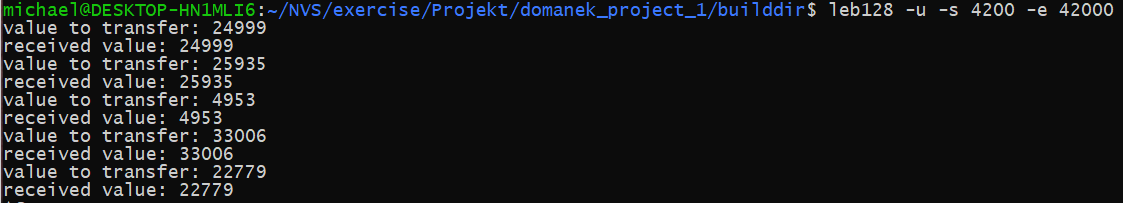
\includegraphics[width=\linewidth]{Konsole}
\caption{Beispiel eines Aufrufs auf der Konsole}
\end{figure}

\begin{figure}[h]
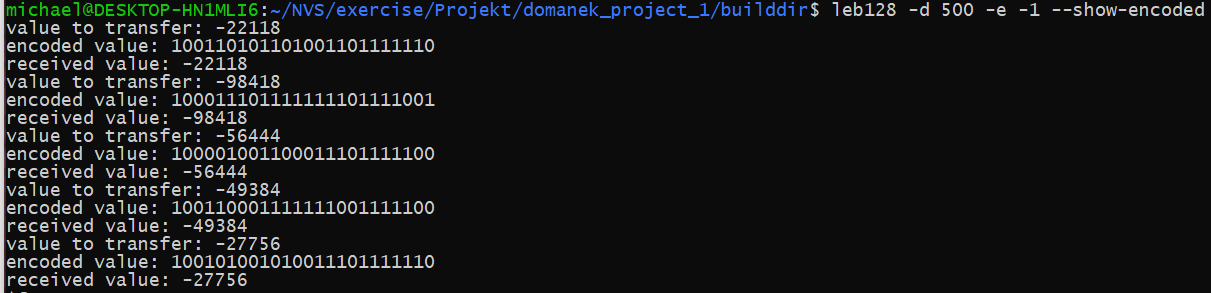
\includegraphics[width=\linewidth]{Konsole2}
\caption{Beispiel eines Aufrufs auf der Konsole}
\end{figure}

\begin{figure}[h]
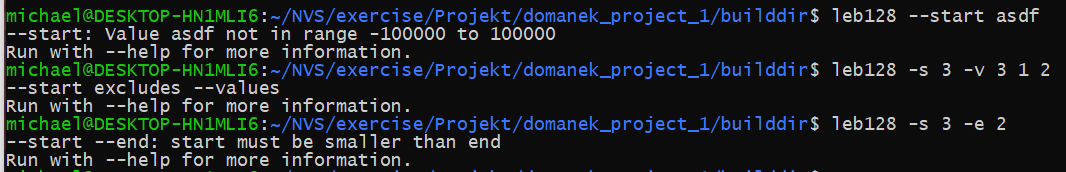
\includegraphics[width=\linewidth]{KonsoleFehler}
\caption{Beispiel von Aufrufen mit Fehler auf der Konsole}
\end{figure}

\subsection{Beispiel mit TOML Konfigurationsfile und JSON Outputfile}
Befehl: \textbf{leb128 \twodashes toml-path ../examples/example-configuration2.toml}

Wenn man diesen Befehl eingibt und nach 2 Übertragung stoppt erhält man folgendes JSON.

\begin{lstlisting}[caption={TOML-Konfigurationsfile}, captionpos=b, frame=single, identifierstyle=\color{black}]
json-output-name = "toml.json"
values = [
  1,
  42,
  7007
]
\end{lstlisting}

\begin{lstlisting}[language=json,caption={JSON Outputfile}, captionpos=b]
{
    "data": [
        {
            "received": 1,
            "transfered": 1
        },
        {
            "received": 42,
            "transfered": 42
        }
    ],
    "delay": 1000,
    "show-encoded": false,
    "unsigned": false,
    "values": [
        1,
        42,
        7007
    ]
}
\end{lstlisting}

\subsection{Auschnitt aus dem Logfile}

Die Zeit wurde nach dem nach dem erste Befehlt ausgeschnitten, damit die Zeile nicht zu lang wird

\begin{lstlisting}[caption={Auschnit aus dem Logfile}, captionpos=b, basicstyle=\small, frame=lines]
[error] [thread 680] --start --end: start must be smaller than end
[2021 01 10 23:07:17,047] [info] [thread 633] ====================
[info] [thread 633] stared new simulation of data transfer with LEB128
[debug] [thread 634] Convert to signed LEB128
[debug] [thread 634] Number: 126
[debug] [thread 634] Binary number: 01111110
[debug] [thread 634] Binary with sign: 00000001111110
[debug] [thread 634] Binary with translated positions: 1111111000000000
[debug] [thread 635] Convert signed LEB128 to decimal
[debug] [thread 635] LEB128 encoded binary: 1111111000000000
[debug] [thread 635] Binary with translated positions: 00000001111110
[debug] [thread 635] Binary number: 1111110
[debug] [thread 635] Number: 126
\end{lstlisting}

\end{document}


